\documentclass[dvipdfmx, tikz]{standalone}
\usepackage{tikz}
\usetikzlibrary{calc,decorations.pathreplacing,quotes,positioning,shapes,fit,arrows,backgrounds,tikzmark}

\begin{document}
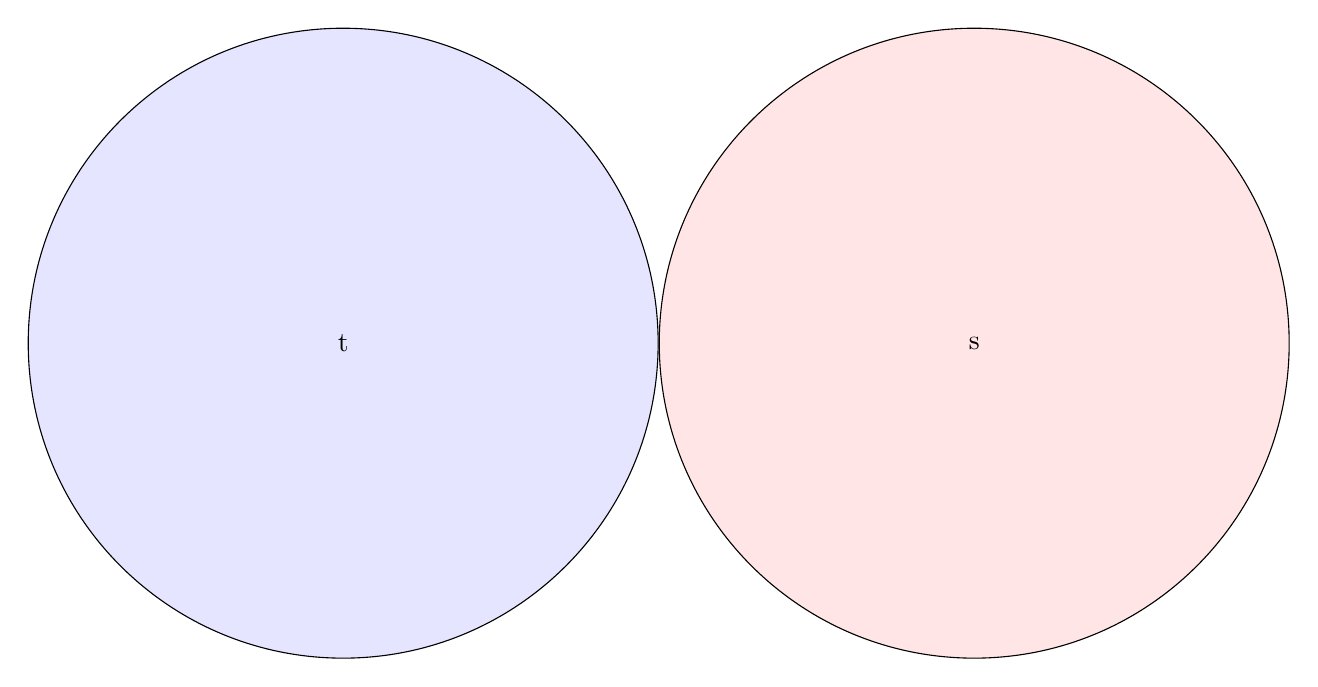
\begin{tikzpicture}[every node/.style={circle, draw, fill=blue!10, minimum size=8cm}, node distance=0cm]
	\node (a1) {t};
	\node (a2) [fill=red!10, right=of a1] {s};
\end{tikzpicture}
\end{document}
